\chapter{Evaluating Quality of Assemblies}

As shown in earlier chapters assembly algorithms are mostly
heuristics with almost zero guaranties. 
Result of the assembly are usually input data into several next steps
of the genome analysis (like finding genes, calculating evolutionary history, ...).
Because of this, any errors in assembly process will have impact on further analysis.
Also sometimes we have access to several variants of the assembly and we need
to choose the best one.
Thus it is important to evaluate quality of the resulting assembly.

Evaluating quality of an assembly is usually hard problem,
since we do not have access to the correct answer.
Due to this we usually resort to use inaccurate indicators, which
give as at least some idea about assembly quality.

In this chapter we give overview of several techniques and statistics
for evaluating assembly. We start with simple indicators based
only on assembly. We also describe indicators based on assembly and correct
answer (which we have if we are benchmarking assemblers). 
There are lots of statistics based on mapping reads to assembly. We first give
overview on mapping reads to assembly and then describe REAPR, which is a tool
for evaluating assembly. We finish chapter with description
of probabilistic models for sequence assembly.

\section{Basic Statistics}

\subsection{Statistics Based Only on Assembly}

To evaluate continuity of the assembly, it is vital
to look into distribution of length of contigs.

There are many ways to look at the distribution of contigs.
We give a brief overview of metrics used in QUAST \citep{Quast}, which
is a standard tool for evaluation of assemblies.

First, we usually look at total length of contigs. We can have expected assembly 
length from other sources so if we the total length of contigs is far from expected
value, we can already see a problem with assembly.
Number of contigs gives us approximate notion of fragmentation of assembly.
Sometimes it is better to look at number of contigs longer than $x$ -- where usually $x = 1000$,
since very small contigs are usually some artefact of the assembly process.
Other statistics for contig length distribution include:
length of the largest contig and $Nx$ (where $0 < x \leq 100$):
the largest contig length $L$, such that using contigs
of length $\geq L$ account for at least $x \%$ of the bases of the assembly.

Note that each of this statistics can be "gambled" so comparing assemblies based
on this statistics can be only done when we assume, that assembly software does only
reasonable operations. This often happens in practice, for example
\citet{gage} shows in his experiments that some assemblers have
higher N50 but also higher number of errors. 

\subsection{Statistics Based on Assembly and Reference Sequence}

Sometimes (especially during evaluation of assembly algorithms) we have access to 
the true sequence
(or almost true sequence), and we can compute various statistics which tell us, how many
errors are in our assembly.
Calculating these statistics usually starts with aligning the assembly to the
reference genome, which
gives us information in the form:
"Substring of the assembly starting at position $a$ and ending at position $b$ can be mapped
to the substring of the reference genome starting at $c$ and ending at $d$ with $e$ edits."
We called these aligned substrings blocks. 

After finding aligned blocks we process to find missassemblies (places with assembly errors).
Missassebly \citep{Quast} is defined as a position in the assembly where block on the left
aligns over $1000$ bases away from the block on the right in the reference,
or blocks align to the opposite strands or to different chromosomes.

Now we can count the number of missassemblies and number of contigs containing missassembly.
We can also look for small differences and count the number of single base difference, either
substitutions, or insertions, or deletions. 
We can also introduce metrics similar to $Nx$, called $NAx$, which is computed in a same way
as $Nx$, but before computing this statistics, we break contigs at missassemblies.

\begin{table}
\centering
\begin{tabular}{|c|c|c|c|c|}
\hline
\multirow{2}{*}{Assembler} & No. of  & N50        & No. of         & NA50  \\
                           & contigs & (thousands)& missassemblies & (thousands) \\\hline
ABySS & 246 & 34 & 1 & 28 \\\hline
Allpaths-LG & {\bf 12} & {\bf 1092} & {\bf 0} & {\bf 1092} \\\hline
SGA & 456 & 208 & 0 & 208 \\\hline
Velvet & 45 & 762 & 17 & 126 \\\hline
\end{tabular}
\caption{Comparison of several assemblers on Staphylococcus aureus dataset. Note that some
  assemblers produce quite high $N50$, but also produce many missassemblies, and their
$NA50$ is much lower.} 
\label{tab:gage}
\end{table}

To provide example of usage of these metrics, we show table (see Table \ref{tab:gage}) from GAGE \citep{gage}, which
benchmarks performance of several assemblers.

\section{Read Mapping}

Many techniques for evaluating assembly rely on finding
positions of original reads in the assembly. This process is often called read mapping.
In this section we give a brief  overview of algorithms and tools used for read mapping.

The goal of the read mapping is to find positions in the DNA sequence where the read might have
originated from. We usually attempt to find positions with the smallest edit distance, 
but sometimes we use more complicated metrics, mostly due to prevalence of specific types of errors in reads.
Formally, we can state that given DNA sequence $S$ and read $R$, the goal of the read mapping
is to find a substring $T$ of $S$ such that the edit distance between $R$ and $T$ is as small as possible.

The exact algorithms for read mapping are variants of a classical dynamic programming algorithms
for finding edit distance of two strings, like Smith-Watterman algorithm (\cite{sm}).
In particularly, we are calculating numbers $T[i][j]$ where $T[i][j]$ is the lowest possible edit
distance between some suffix of $S[0..i-1]$ and $R[0..j-1]$. 
We put:
$$T[i][0] = 0$$
$$T[i][j] = \min(T[i-1][j] + 1, T[i][j-1] + 1, T[i-1][j-1] + S[i-1] \neq R[j-1])$$

Extracting mapping from this matrix is a straightforward task.
Unfortunately, finding mapping for one read using this algorithm takes $O(|S||R|)$ time,
which is too much considering that the DNA sequence is typically millions bases long and we usually have
a few million reads.

Practical algorithms for read mapping can be divided into two types:
hash based seed-and-extend algorithms and algorithms based on suffix arrays and their extensions.

Hash based algorithms are based on an observation that if we put upper bound on number
of errors in read, there exists
some substring of read of length at least $k$ that is conserved without errors,.
These conserved substrings are called seeds. 
We can exploit this by indexing the DNA sequence 
and then finding all possible seeds matches for read.
This is usually done using hash tables. After finding seeds we use the
dynamic programming on a small area around the seed location.
Examples of tools using this approach 
include BLAST, BLAT, and many others \citep{blast,blat}.

Nowadays, lots of read mappers uses extension of suffix arrays called FM-index
\citep{fmindex, fmindex2}, which we will now describe.

\paragraph{Burrows-Wheeler transform.} Given sequence $S = s_1 s_2 \dots s_n$, where
$s_n = \$$. Burrows-Wheeler transform (BWT) of $S$ is constructed
by lexicographically ordering all cyclical rotations of $S$ and then
taking last characters from each rotations.
Formally, if $S_i$ is rotation starting at $i$-th positions of $S$ and array
$X_i$ is index of $i$-th lexicographically smallest rotation, the
BWT of $S$ is sequence $B = S_{X_1}[n] S_{X_2}[n] \dots S_{X_n}[n]$.
Using standard algorithms for construction of suffix array we
can construct BWT of $S$ in $O(|S|)$ time and space.

\paragraph{Indexing using BWT.}
BWT can be used to find an occurrence of string $P$ in $S$ as a substring.
Denote $C(a)$ as the smallest index $i$ where $S_{X_i}[0] = a$ (it is also
a total number of characters smaller than $a$ in $S$).
Denote $Occ(a,i)$ as the number of occurrences of $a$ in $B[1], \dots, B[i]$.
The goal of the indexing is to find an interval $(b, e)$ such that
$b$ is the smallest number where $P$ is a prefix of $S_{X_b}$
and $e$ is the largest number where $P$ is a prefix of $S_{X_e}$.
If we know the interval $(b, e)$ for $P$, then the interval for
$aP$ is given as:
$$(C(a) + Occ(a, b - 1) + 1, C(a) + Occ(a, e))$$

By starting from an empty string, we can use
this formula to calculate interval for any pattern, building
it from the end of pattern. Note that
the interval for empty string is $(1, |S|)$.
We can also implement
a backtracking to allow for inexact matching of the pattern. 
Improved algorithms for inexact matching are described by \citet{fmindex3}.

To achieve good space complexity, we use compressed representation
of arrays $B$, $Occ$ and $C$, and some samples from array $X$ (we can reconstruct
array $X$ using samples and data from $B$). 
Examples of FM-index based read mappers are Bowtie2, BWA and SOAP
\citep{bowtie2,fmindex,soap}.

\section{REAPR}

If we have access to original reads and the assembly we can find locations
of this reads in the assembly and then compute several statistics which
can point out to suspicious regions in the assembly.
This is needed since assemblers use various heuristics and sometimes discard
some information from reads. 

There are several tools which do this, one of them is REAPR (\cite{Reapr}) which we describe
in more detail below.

REAPR is designed for working with paired reads, so in the following we will assume that
we have a single library of paired reads.
REAPR starts by mapping reads to the assembly, i.e. for each read we know locations it the assembly
and the edit distance for this mapping.

After mapping step, we can calculate following metrics for each base in the assembly:
\begin{itemize}
\item Read coverage: how many reads are mapped to current position. Low coverage usually indicates assembly error.
\item Type of read coverage: we can calculate read coverage for specific conditions such as reads without pairs,
reads with pair with wrong orientation, coverage for reads which map with or without reverse complementing.
\item Read clipping: sometimes read can be mapped to assembly but a few bases at the end of the reads do not match.
We call reads mapped this way as soft-clipped.
At each base, we count the number of soft-clipped reads starting or ending at this base. A high read
clipping count can be sign of insertion of deletion in the assembly.
\item Paired coverage: same as read coverage, but we treat properly paired reads as a one long read when calculating coverage.
\item FCD error: At each base we construct a plot of coverage distribution of bases
  only from pairs which cover given base. The difference between the expected
  and observed distribution, called FCD errors, is is measured by taking the area between the two plots (see Fig. \ref{fig:fcd}).
\end{itemize}

\begin{figure}
\centering
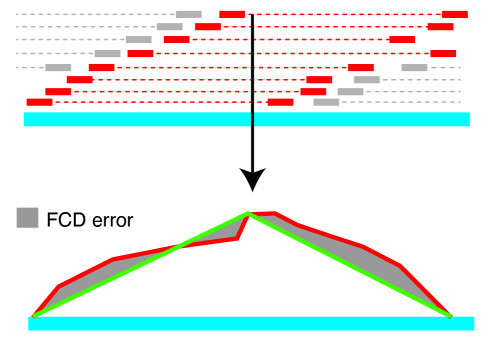
\includegraphics{../figures/fcd.jpg}
\caption{Example of calculating FCD errors. Fragments covering given base
shown in red, are used to construct coverage depth plot (red). The FCD error is the
area (grey) between the observed (red) plot and ideal (green). Image taken
from \citet{Reapr}.}
\label{fig:fcd}
\end{figure}

REAPR uses this metrics to calculate score at each base 
(the score calculation is ad hoc algorithm) and then breaks assembly
at places with low score.

\section{Probability Models}
\label{sec:prob}
In some cases, we have to compare multiple assemblies and decide which one is
the best. This can be done using various criteria, but \cite{Ghodsi2013} shows
that a very simple and theoretically sound probabilistic model can do the job.

In general, the probabilistic model defines the probability $\Pr(R|A)$ that a set of
sequencing reads $R$ is observed assuming that the assembly $A$ is the
correct assembly of the genome. Since the sequencing itself is a
stochastic process, it is very natural to characterize concordance of
reads and an assembly by giving a probability of observing a particular
read.

\def\LAP{\mathrm{LAP}}

\paragraph{Basics of the likelihood model.}
The model assumes
that individual reads are independently sampled, and thus the overall
likelihood is the product of likelihoods of the reads:
$\Pr(R|A) = \prod_{r\in R} \Pr(r|A).$
To make
the resulting value independent of the number of reads in set 
$R$, we use as the main
assembly score the log average probability of a read computed as
follows: $\LAP(A|R) = (1/|R|)\sum_{r\in R} \log \Pr(r|A).$ Note that
maximizing $\Pr(R|A)$ is equivalent to maximizing $\LAP(A|R)$.

If the reads were error-free and each position in the genome was
sequenced equally likely, the probability of observing read $r$
would simply be $\Pr(r|A)=n_r/(2L)$, where $n_r$ is the number of 
occurrences of the read as a substring of the assembly $A$,
$L$ is the length of $A$, and thus $2L$ is the length of the two
strands combined.

Other way of looking at the error free model is to say that probability
of generating read from position $j$ is one if read exactly matches 
assembly at given position and zero otherwise. This can be extended
to account for sequencing errors. The probability of generating read
from position $j$ is a real number which represent likelihood of generating
that read from given position. This value mainly depends on the number
of differences between read and assembly at the specific position.

Formally we define $p_{r, j}$ as probability of generating read $r$ from a sequence
that ends at position $j$. Then the probability of generating read $r$ can be computed as:

$$\Pr(r|A) = \frac{\sum_j p_{r,j}^{forward} + \sum_j p_{r,j}^{reverse}}{2L}$$ 

The individual probabilities $p_{r,j}$ can be computed via dynamic programing, where
we define $T[x,y]$ as a probability of generating prefix of read of length $y$ from sequence
which ends at position $x$. Clearly $p_{r,j} = T[j, \ell]$, where $\ell$ is the length
of the read. Also $T[x,0] = 1$ for all $x$ and $T[0,y]= 0$ for all $y > 0$.
The other probabilities can be computed using following formula:
$$T[x,y] = T[x-1,y-1]\Pr(Subs(A[x], r[y])) + T[x,y-1]\Pr(Ins(r[y])) +
T[x-1,y]\Pr(Del(A[x]))$$

Where $A[x], r[y]$ represents bases at the assembly at position $x$ and in read at
position $y$ respectively and $Subs, Ins, Del$ represents events of substitution, insertion
and deletion.

However this dynamic programming is too time consuming. 
In practice it is good enough to align reads to the assembly and to compute
likelihood from the alignments.
Given read $r$ and 
a set $S_r$ of a few best alignments of $r$ to
genome~$A$, as obtained by one of standard fast read alignment tools, the
probability of generating read $r$ can be estimated as:
\begin{equation}
\Pr(r|A)\approx \frac{\sum_{j\in S_r} R(s_j, m_j)}{2L},
\end{equation}
where $m_j$ is the number of matches in the $j$-th alignment, and
$s_j$ is the number of mismatches and indels implied by this alignment.

\paragraph{Paired reads.}
Likelihood model can accommodate also paired reads.
We assume that the insert size distribution in a set of reads $R$ 
can be modeled by the normal
distribution with known mean $\mu$ and standard deviation $\sigma$.
The probability of observing paired reads $r_1$ and $r_2$ 
can be estimated from the sets of alignments $S_{r_1}$ and $S_{r_2}$ as follows:

\begin{equation}
\Pr(r_1, r_2|A) \approx 
\frac{1}{2L}
\displaystyle\sum_{j_1 \in S_{r_1}} 
\displaystyle\sum_{j_2 \in S_{r_2}} 
R(s_{j_1}, m_{j_1}) R(s_{j_2}, m_{j_2})
\Pr(d(j_1, j_2)|\mu, \sigma)
\end{equation}
As before, $m_{j_i}$ and $s_{j_i}$ are the numbers of matches and
sequencing errors in alignment $j_i$ respectively, 
and $d(j_1,j_2)$ is the distance between the two alignments
as observed in the assembly. 
If alignments $j_1$ and $j_2$ are in two different contigs,
or on inconsistent strands, $\Pr(d(j_1, j_2)|\mu, \sigma)$ is zero.

\paragraph{Reads that have no good alignment to $A$.}
Some reads or read pairs do not align well to $A$, and as a result, their
probability $\Pr(r|A)$ is very low; our approximation by a set of
high-scoring alignments can even yield zero probability if set $S_r$
is empty.  Such extremely low probabilities then dominate the log
likelihood score. \citet{Ghodsi2013} propose a method that assigns
such a read a score approximating the situation when the read would be
added as a new contig to the assembly. In practice this usually
means having lower bound on the probability of generating a read.

To illustrate usufullness of likelihood we present
few results from \citet{Ghodsi2013} where we compare
several assemblers and resulting $NA50$ and assembly likelihood,
and show that there is a good correlation between this measures (see Table
\ref{tab:like}). More data can be found in \citet{Ghodsi2013}.

\begin{table}
\centering
\begin{tabular}{|c|c|c|c|}
\hline
Assembler & LAP & N50 (thousands) & NA50 (thousands) \\\hline
Reference sequence & $-23.509$ & 2873 & 2873 \\\hline
AbySS & $-24.584$ & 34 & 28 \\\hline
Allpaths-LG & $-23.760$ & 1092 & 1092 \\\hline
SOAPdenovo & $-23.862$ & 332 & 288 \\\hline
Velvet & $-23.925$ & 762 & 126  \\\hline
\end{tabular}
\caption{Comparison of several assemblers on Staphylococcus aureus dataset
using LAP and NA50.}
\label{tab:like}
\end{table}

There are also other approach to calculate assembly likelihood
most notably ALE and CGAL \citep{ALE, CGAL}.

\section{Summary}

In this chapter we provided overview of assembly evaluation techniques.
We showed several basic measures for assembly (like $N50$, $NA50$),
provided insight into mapping reads on assembly and how to use
read mapping to find suspicious regions in assembly using REAPR.
We also demonstrated that likelihood models are good and simple
tools to compare several assemblies.

